\documentclass{article}

\usepackage{fullpage}
\usepackage{graphicx}
\usepackage{subfigure}

\begin{document}

\section{Sleeve measurements}

\paragraph{Overarm length}
Measure from shoulder tip (1/4 inch from the end of shoulder. If you start to raise your arm, a hollow will form at the shoulder joint. This is shoulder tip – approximately) to 1/2 inch past wrist bone. Be sure to measure with arm slightly bent or else sleeve will appear too short when fully bent or too long when fully relaxed.

\paragraph{Elbow length}
Shoulder tip to bone at elbow.

\paragraph{Bicep}
Measure around the arm and ensure measuring tape is level with the armhole depth/armpit (click here to find armhole depth/armpit). Add 1 inch to this measurement (for ease).

\paragraph{Wrist}
Measure around the widest part of the hand.


\begin{figure}[!htp]
\centering
	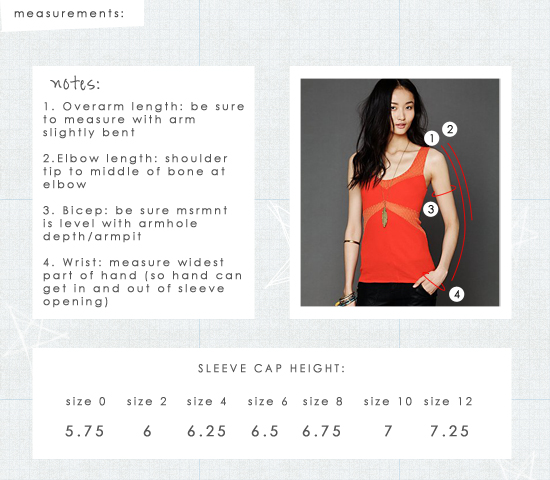
\includegraphics[width=0.6\textwidth]{slv-measurements.jpg}
\end{figure}


\section{Front measurements}

\paragraph{Full length}
Shoulder at neck to waist line.

\paragraph{CF (center front) length}
Hollow at center front neck to waist line.

\paragraph{Shoulder tip}
1/4 inch from the end of shoulder (if you start to raise your arm, a hollow will form at the shoulder joint. This is shoulder tip – approximately).

\paragraph{Shoulder length}
Shoulder at neck to shoulder tip.

\paragraph{Across shoulder}
Shoulder tip to shoulder tip – MEASURED on back – and DIVIDED by 2 (across shoulders for both front and back bodice sloper is taken on back).

\paragraph{Armhole depth}
Shoulder tip to armpit (usually 1/2 inch to 1 inch below actual armpit). Using two l-square rulers, arrange rulers as shown in diagram and measure. This measurement is the most often incorrectly measured measurement. Because of this, I suggest to cross check this measurement two ways. One way is to measure the armhole from shoulder tip to bottom of armhole on a very good fitting sleeveless blouse (measure straight and not measure along the curve). Another way to cross check this measurement is to compare it to standard measurements. If the standard armhole depth for a size 6 is 7.25 inch and armhole grades 0.25 inch per size, use math to find the standard armhole depth for your size. Are both of these measurements close to the armhole depth measurement taken on body?

\paragraph{Bust depth}
Shoulder tip to bust point (bust point is the nipple. To find, poke a needle from INSIDE of bra/tank top to OUTSIDE and mark.

\paragraph{Bust span}
Bust point to bust point, divided by 2.

\paragraph{Bust arc}
CF to bust point to armhole depth/side seam. Do not measure from CF to bust point and then pivot measuring tape up to armhole/side seam because the hollow in between breasts cause the measurement to be larger/bigger, especially if your breasts are very large. In theory, this measurement should be taken from the bridge between bust points at CF but this is very hard. Measure instead from bust point to armhole/side seam and then add this measurement to bust span measurement (make sure that bust span measurement is 1/2 of bust point to bust point).

\paragraph{Shoulder slope}
CF waist line to shoulder tip. Be sure that to keep measuring tape taut and extend it straight from waist, over bust point, and to shoulder tip.

\paragraph{Side seam (SS) length}
Armhole depth to waist line.

\paragraph{Waist arc}
CF to SS along waist line.


\section{Back measurements}


\begin{figure}[!htp]
\centering
\subfigure
{
	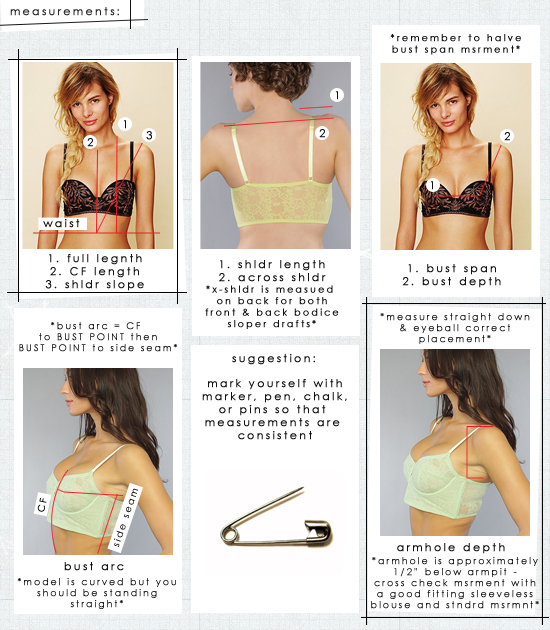
\includegraphics[width=0.6\textwidth]{front-measurements.jpg}
}

\subfigure
{
	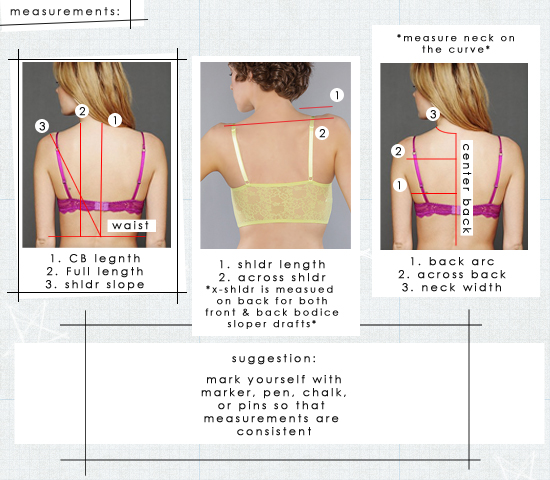
\includegraphics[width=0.6\textwidth]{back-measurements.jpg}
}
\end{figure}


\paragraph{Full length} Shoulder at neck to waist line.

\paragraph{Center back (CB) length} Prominent bone at nape of neck (top of back neck) to waist line.

\paragraph{Shoulder slope} CB waist line to shoulder tip. Be sure to keep measuring tape taut and to extend it straight from waist to shoulder tip.

\paragraph{Back neck} Tie a chain/tie/elastic loosely around the neck and allow it to rest at the neck base. Then measure from CB neck (prominent bone at the nape of the neck) to shoulder seam along curve.

\paragraph{Back arc} CB to side seam/AH (ensure that measuring tape in level and perpendicular to armhole base/CB line).

\paragraph{Across back} CB line to armhole at approximately 5 inch down from shoulder seam/neckline (remember to mark armhole line with marker, pen, pins, etc). A way to cross check this measurement is to subtract 1/2 inch from across shoulders. Example: If your across shoulders is 14 inch, is your across back in the range of 13.25--13.5 inch? Across back and across shoulders have a standard relationship that ensures the armhole is a smooth curve from shoulder seam to the base of the armhole on both front and back.

\paragraph{Waist arc} CB line to side seam along waist line.


\end{document}